The goal of our evaluation is to demonstrate that our co-design
algorithm achieves near-optimal control cost, but for much smaller representations $\zbottleneck$ compared to task-agnostic methods. 

\tbf{Metrics.} We evaluate the following metrics: 
1) We quantify the \textbf{control cost} for various bottleneck sizes $\zbottleneck$, relative to the \textit{optimal cost} when ground-truth input $s$ is shared \textit{without} a network bottleneck.
2) To quantify the benefits of sending a representation of size $\zbottleneck$ compared to the full forecast $\shat_{t:t+H-1}$ of size $\pH$, we define the \textbf{compression gain} as $\frac{\pH}{\zbottleneck}$. We also compare the minimum bottleneck $Z$ required to achieve within $5\%$ of the optimal cost for all benchmarks. 
3) Since the objective of Prob. \ref{prob:codesign} also incorporates prediction error, we quantify the \textbf{MSE forecasting error} for various $\zbottleneck$.

% \begin{figure*}[t]
\vskip 0.2in
\begin{center}
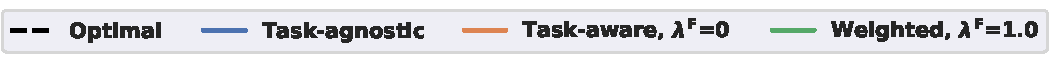
\includegraphics[width=0.8\columnwidth]{figures/main_legend.pdf}
%\subfigure[]{
\subfigure{
{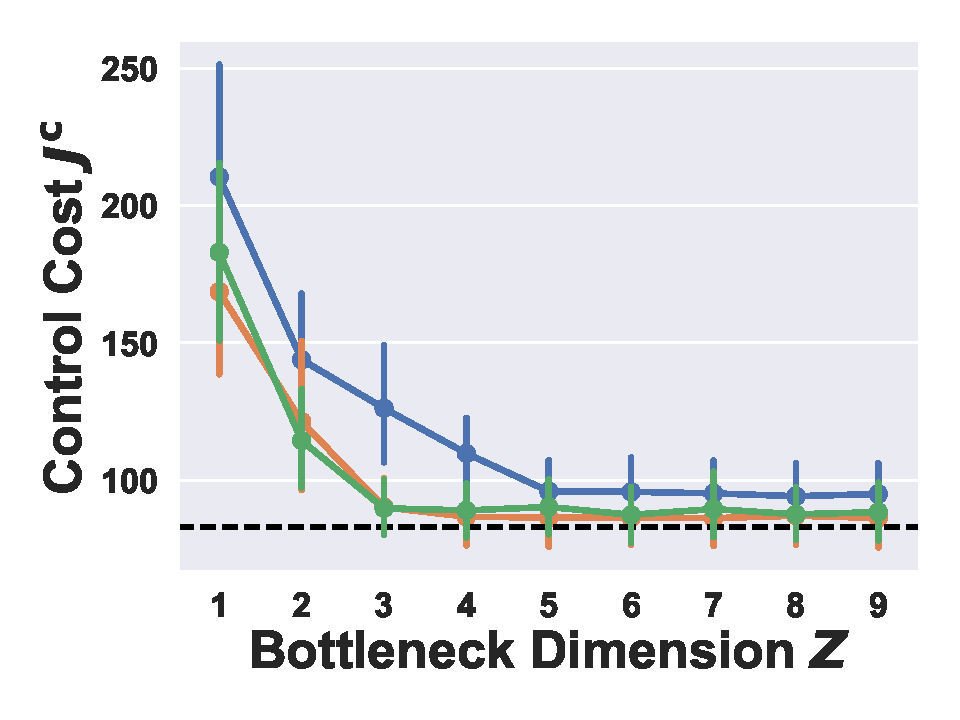
\includegraphics[width=0.31\columnwidth]{figures/iot/iot_cost_bottleneck.pdf}}
\label{fig_iot_cost_bottleneck}
}
%\subfigure[]{
\subfigure{
{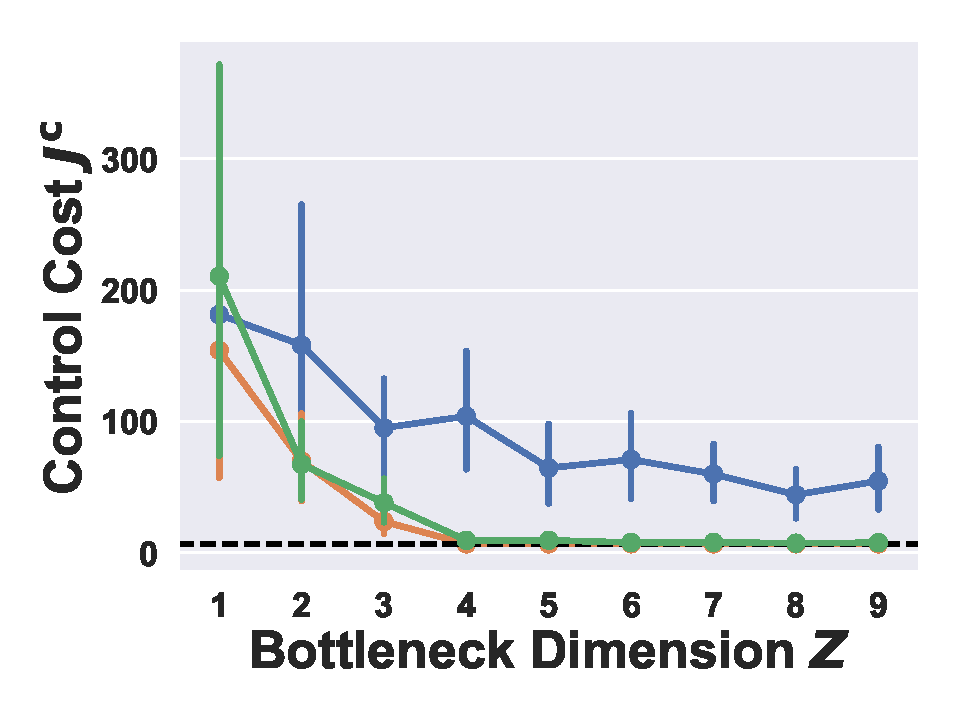
\includegraphics[width=0.31\columnwidth]{figures/cell/cell_cost_bottleneck.pdf}}
\label{fig_cell_cost_bottleneck}
}
%\subfigure[]{
\subfigure{
{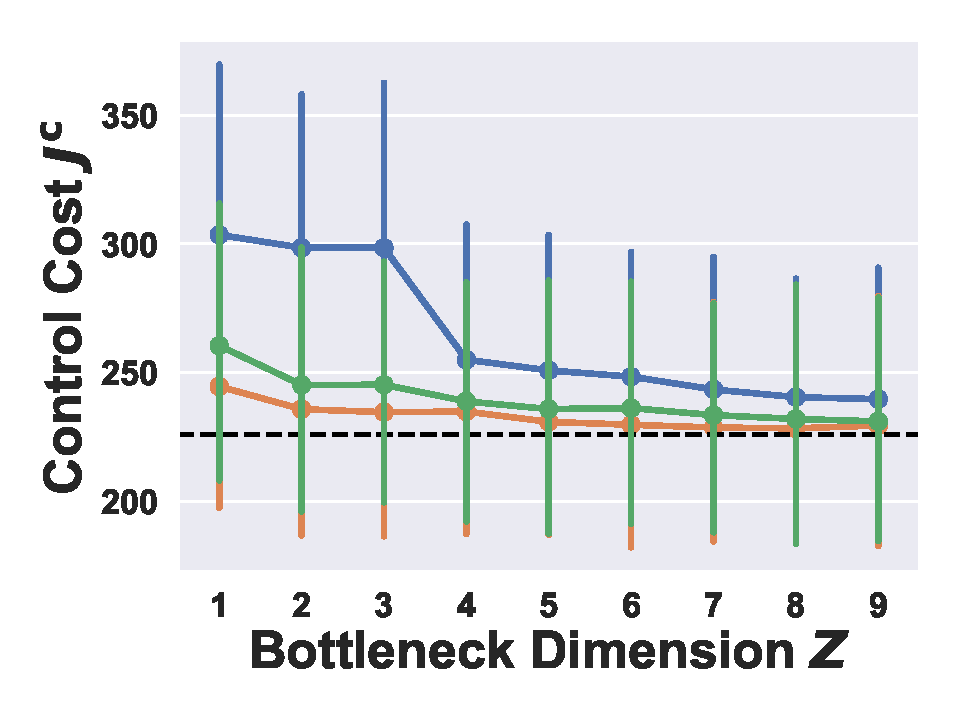
\includegraphics[width=0.31\columnwidth]{figures/pjm/pjm_cost_bottleneck.pdf}}
\label{fig_pjm_cost_bottleneck}
}
%\subfigure[]{
\subfigure{
{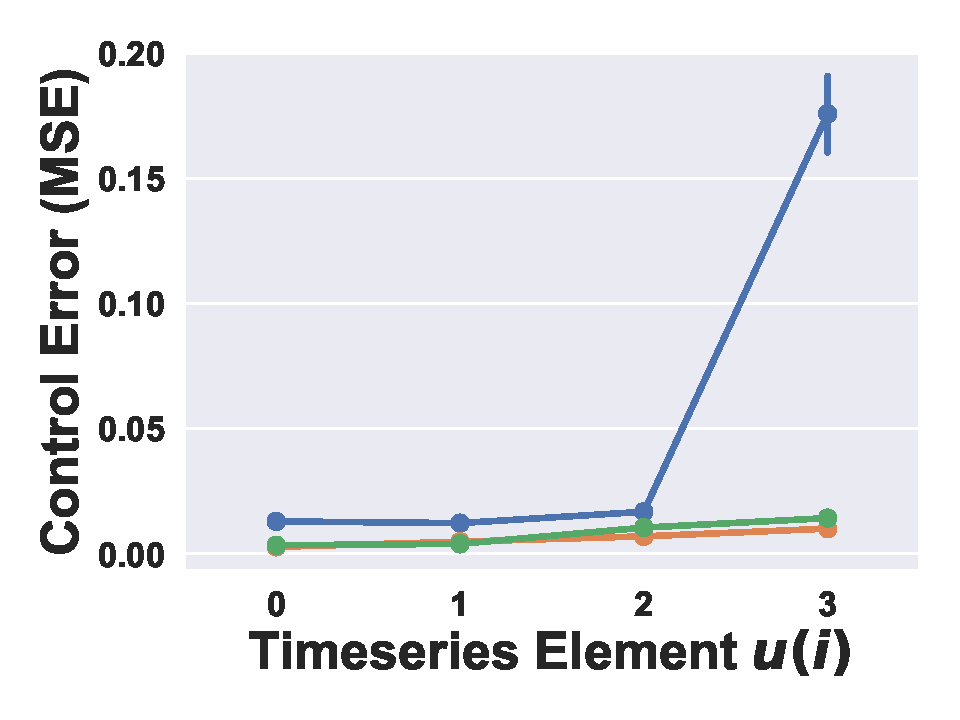
\includegraphics[width=0.31\columnwidth]{figures/iot/control_errors.pdf}}
\label{fig_iot_control_errors}
}
%\subfigure[]{
\subfigure{
{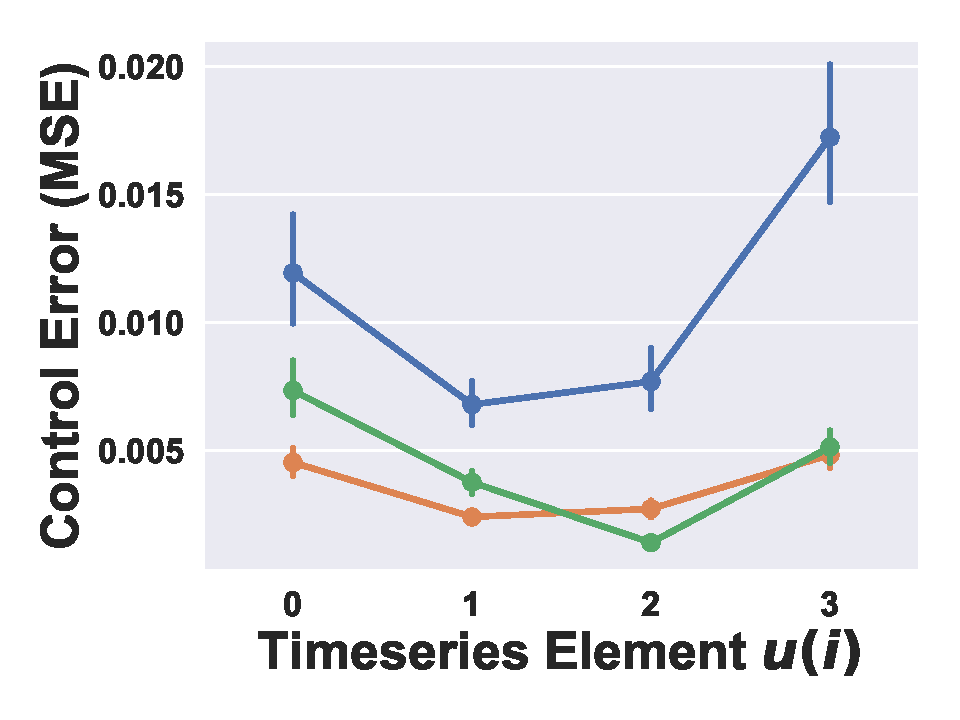
\includegraphics[width=0.31\columnwidth]{figures/cell/control_errors.pdf}}
\label{fig_cell_control_errors}
}
%\subfigure[]{
\subfigure{
{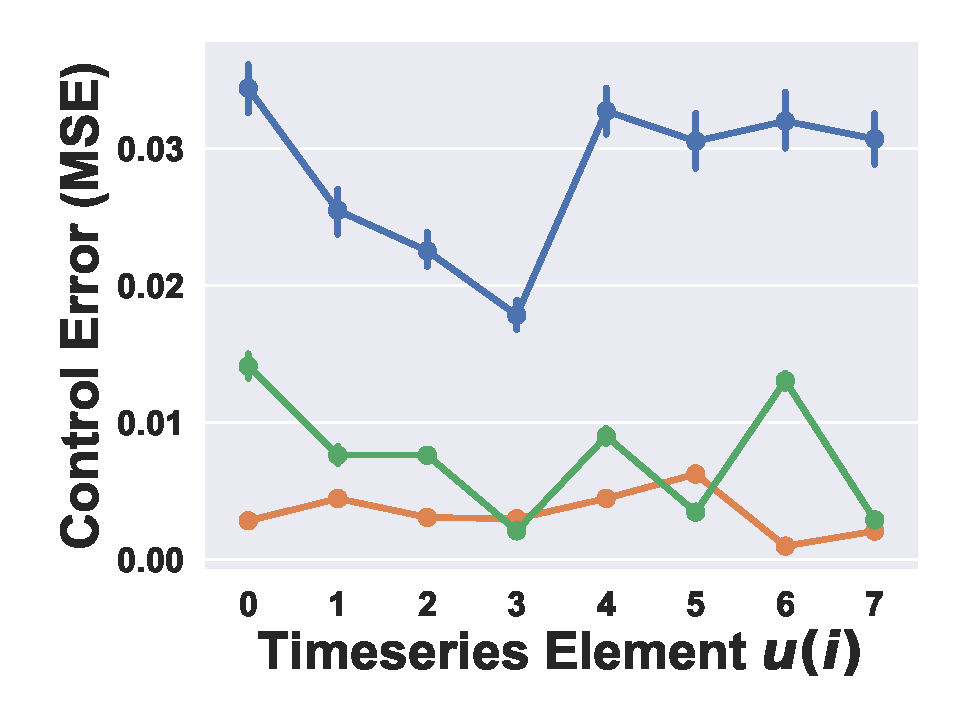
\includegraphics[width=0.31\columnwidth]{figures/pjm/control_errors.pdf}}
\label{fig_pjm_control_errors}
}
%\subfigure[]{
\subfigure{
{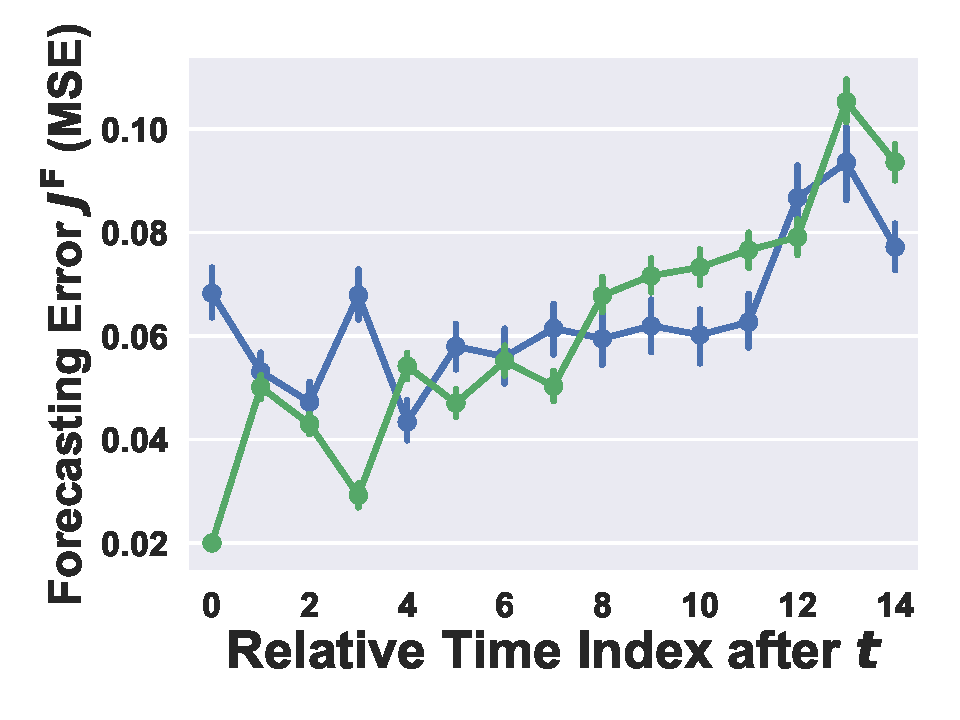
\includegraphics[width=0.31\columnwidth]{figures/iot/forecast_errors_time_horizon.pdf}}
\label{fig_iot_forecast_errors_time_horizon}
}
%\subfigure[]{
\subfigure{
{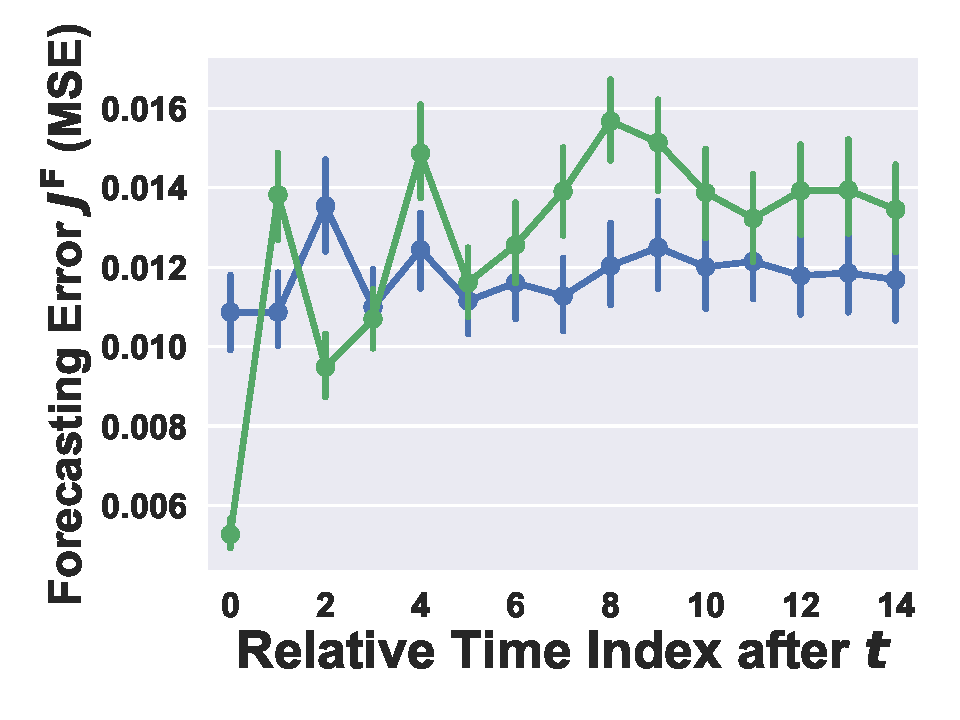
\includegraphics[width=0.31\columnwidth]{figures/cell/forecast_errors_time_horizon.pdf}}
\label{fig_cell_forecast_errors_time_horizon}
}
%\subfigure[]{
\subfigure{
{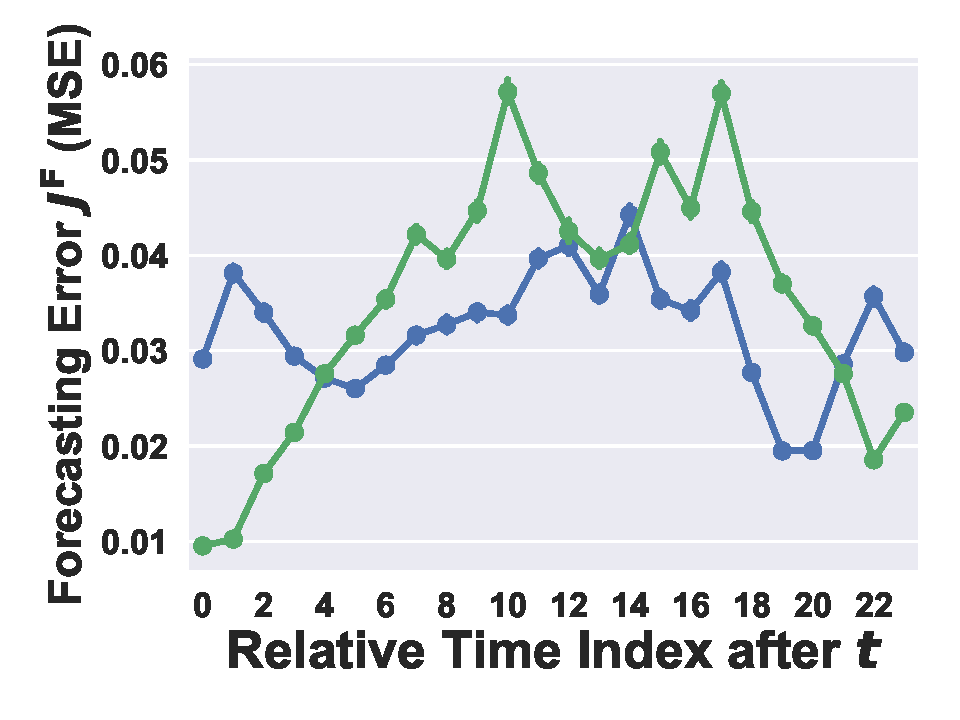
\includegraphics[width=0.31\columnwidth]{figures/pjm/forecast_errors_time_horizon.pdf}}
\label{fig_pjm_forecast_errors_time_horizon}
}
\caption{\textbf{Real-world dataset results: } From left to right, the columns correspond to smart factory regulation from IoT sensors, taxi dispatching with cell demand, and battery storage optimization. \textbf{(Row 1)} Co-design achieves lower cost $\Jcontrol$ for smaller bottlenecks $\zbottleneck$ compared to task-agnostic methods. \textbf{(Row 2)} We also achieve lower error for each dimension $i$ of the vector control, $u(i)$, plotted for a highly-compressed $Z=3$. \textbf{(Row 3)} Co-design heavily reduces forecasting errors for initial horizons that are especially important for MPC's decision-making.}
%While a task-agnostic approach (blue) distributes forecasting errors roughly evenly across a horizon $H$, our co-design approaches heavily reduce errors for initial horizons that are especially important for MPC's decision-making.}
\label{fig_real}
\end{center}
\vskip -0.2in
\end{figure*}
%Aggregated forecasting error for  each relative time index when $Z=3$, under different policies. (j-l) Forecasting error for each $s(i)$ and each relative time index when $Z=3$, under task-agnostic (top) and weighted (bottom) policy, respectively.
%\caption{Results for real data. Columns from left to right corresponds to smart home regulation, taxi dispatching and battery storage optimization, respectively. (a-c) Control cost $J$ under different bottleneck dimension $Z$ and training policies; (d-f) Control error for each $u(i)$ when $Z=3$ under different training policies; (g-i) Aggregated forecasting error for  each relative time index when $Z=3$, under different policies. (j-l) Forecasting error for each $s(i)$ and each relative time index when $Z=3$, under task-agnostic (top) and weighted (bottom) policy, respectively.}


%\subsection{Algorithm Instantiations and Benchmarks}
\tbf{Algorithms and Benchmarks.} We test the above metrics on the following algorithms, which represent various instantiations of Alg. \ref{alg:codesign} for different $\lambdaforecast$ as well as today's prevailing method of optimizing for prediction MSE. Our algorithms and benchmarks are:
1) \textbf{Fully Task-aware ($\lambdaforecast=0$):} We co-design with $\lambdaforecast=0$ according to Alg. \ref{alg:codesign} to assess the full gains of compression.
2) \textbf{Weighted}: We instantiate Alg. \ref{alg:codesign} with $\lambdaforecast > 0$ to assess the benefits of task-aware compression as well as forecasting errors induced by compression. In practice, $\lambdaforecast$ is user-specified. For visual clarity, we show results for $\lambdaforecast=1$ in Fig. \ref{fig_real} since the trends for other $\lambdaforecast$ mirror those in Fig. \ref{fig:main_pca_full}.
3) \textbf{Task-agnostic (MSE)}: Our benchmark learns a forecast $\boldshat$ to minimize MSE prediction error, which is directly passed to the controller \textit{without} any co-design.

\textbf{Forecaster and Controller Models.} 
We compared forecast encoder/decoders with long short term memory (LSTM) DNNs \cite{LSTM} and simple feedforward networks. We observed similar performance for all models, which we hypothesize is because co-design needs to represent only a small set of \textit{control-relevant} features. We used standard DNN architectures, hyperparameters, and the Adam optimizer, as further detailed in the supplement. 
Our code and data are publicly available at \url{https://github.com/chengjiangnan/cooperative_networked_control}.
% \SC{All our code and data (provided in the supplement) will be \textbf{publicly-released} after peer review.}
%Finally, we use differentiable quadratic program solvers to obtain the gradient of MPC's control cost using the \textsc{qpth} \cite{amos2017optnet} library. 

\subsection{Linear Dynamics}
\label{subsec:linear}

\begin{figure*}[t]
\vskip 0.2in
\begin{center}
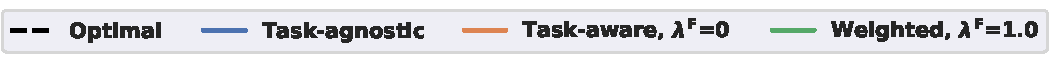
\includegraphics[width=0.8\columnwidth]{figures/main_legend.pdf}
%\subfigure[]{
\subfigure{
{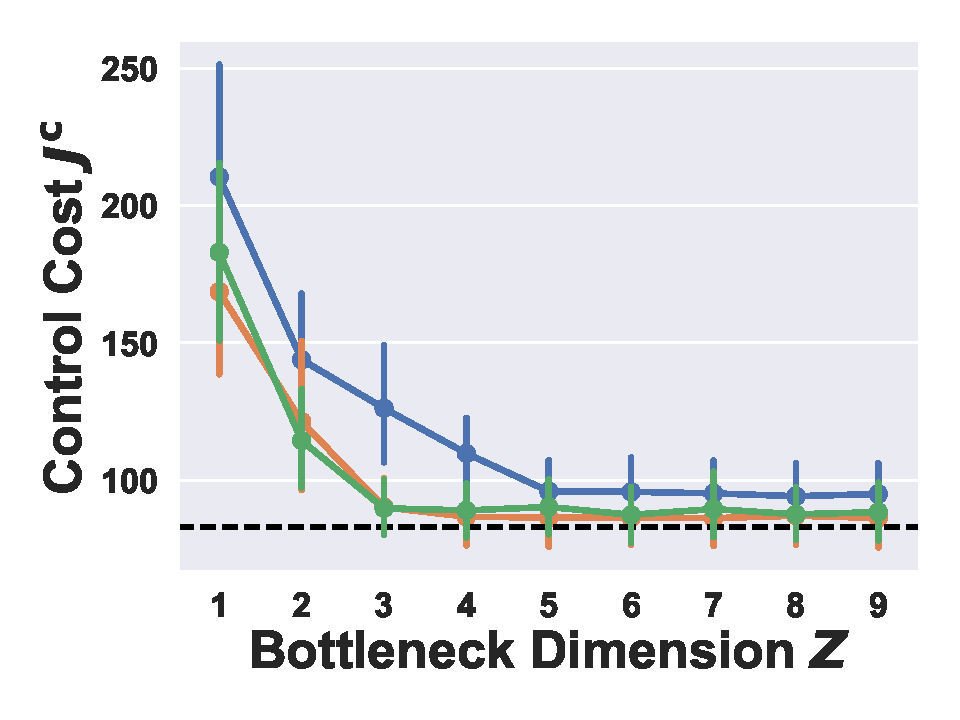
\includegraphics[width=0.31\columnwidth]{figures/iot/iot_cost_bottleneck.pdf}}
\label{fig_iot_cost_bottleneck}
}
%\subfigure[]{
\subfigure{
{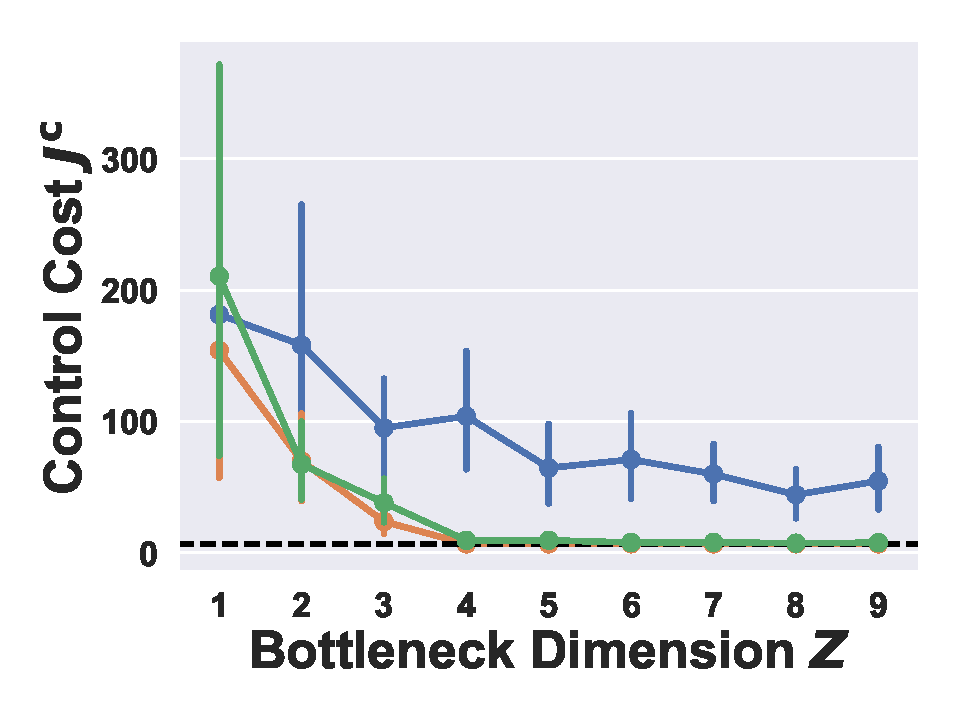
\includegraphics[width=0.31\columnwidth]{figures/cell/cell_cost_bottleneck.pdf}}
\label{fig_cell_cost_bottleneck}
}
%\subfigure[]{
\subfigure{
{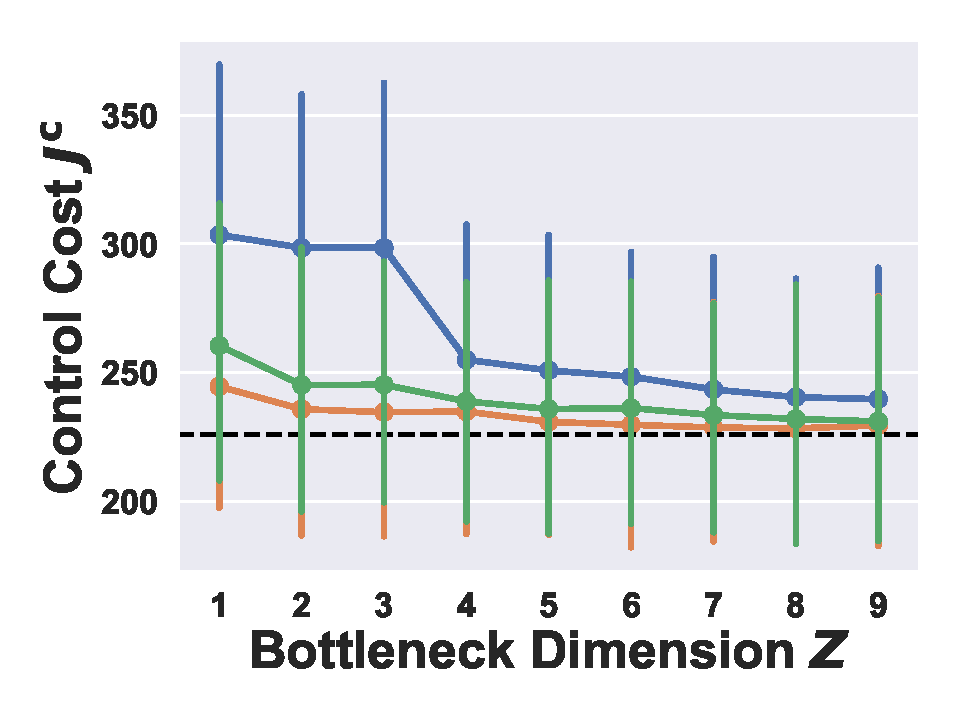
\includegraphics[width=0.31\columnwidth]{figures/pjm/pjm_cost_bottleneck.pdf}}
\label{fig_pjm_cost_bottleneck}
}
%\subfigure[]{
\subfigure{
{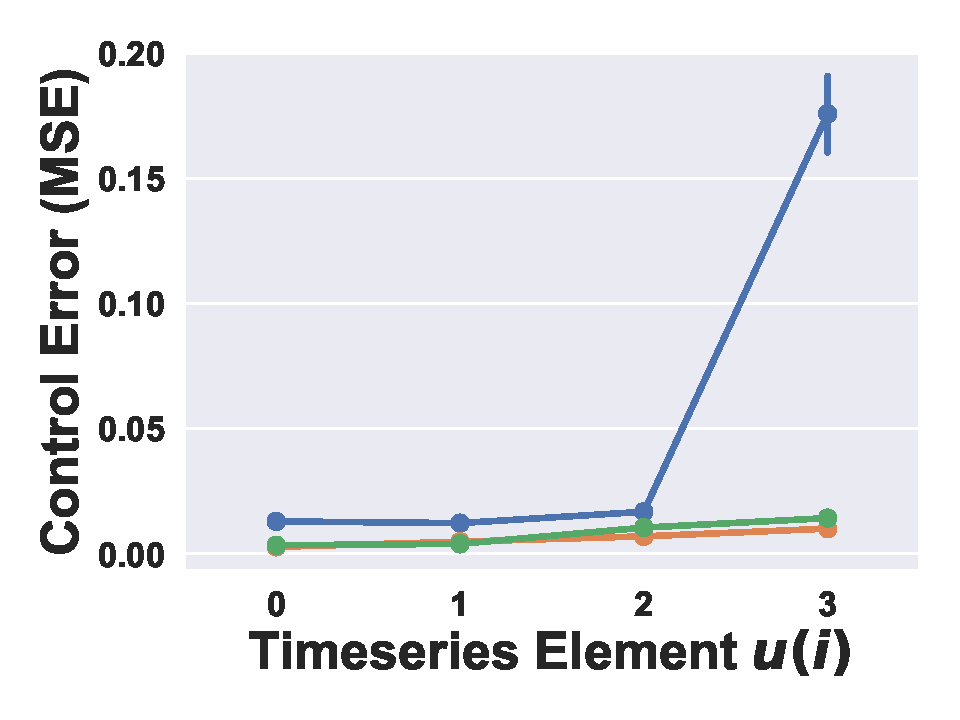
\includegraphics[width=0.31\columnwidth]{figures/iot/control_errors.pdf}}
\label{fig_iot_control_errors}
}
%\subfigure[]{
\subfigure{
{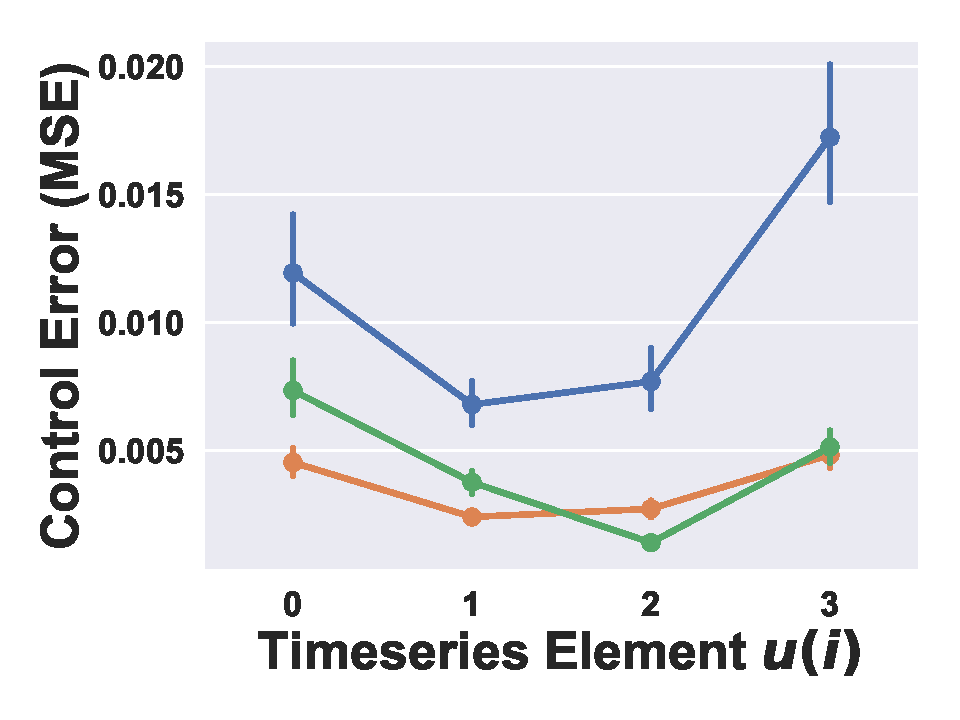
\includegraphics[width=0.31\columnwidth]{figures/cell/control_errors.pdf}}
\label{fig_cell_control_errors}
}
%\subfigure[]{
\subfigure{
{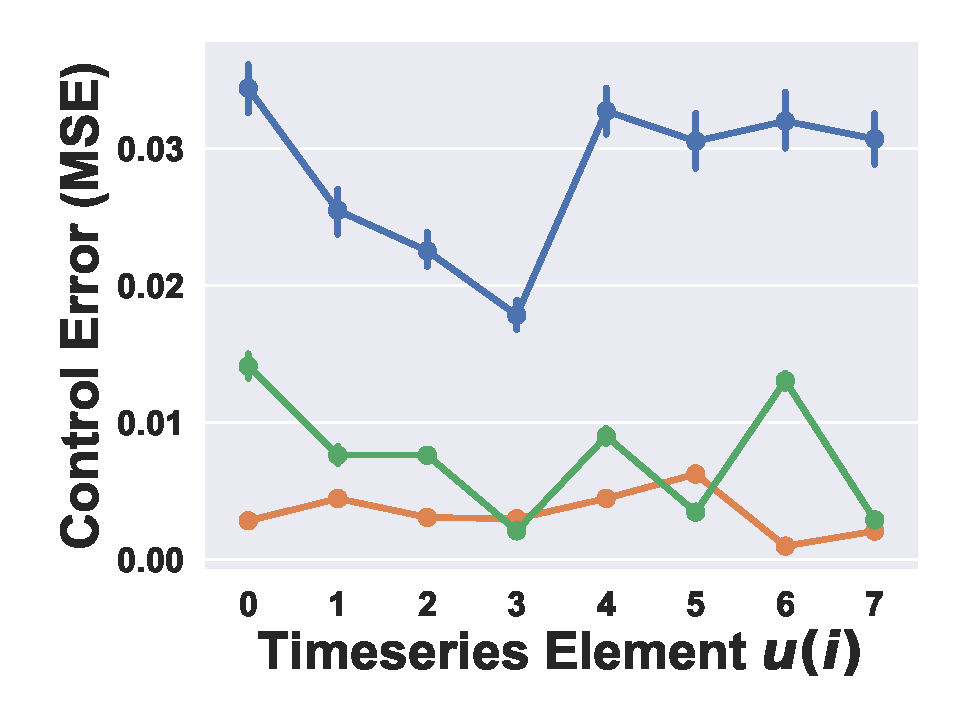
\includegraphics[width=0.31\columnwidth]{figures/pjm/control_errors.pdf}}
\label{fig_pjm_control_errors}
}
%\subfigure[]{
\subfigure{
{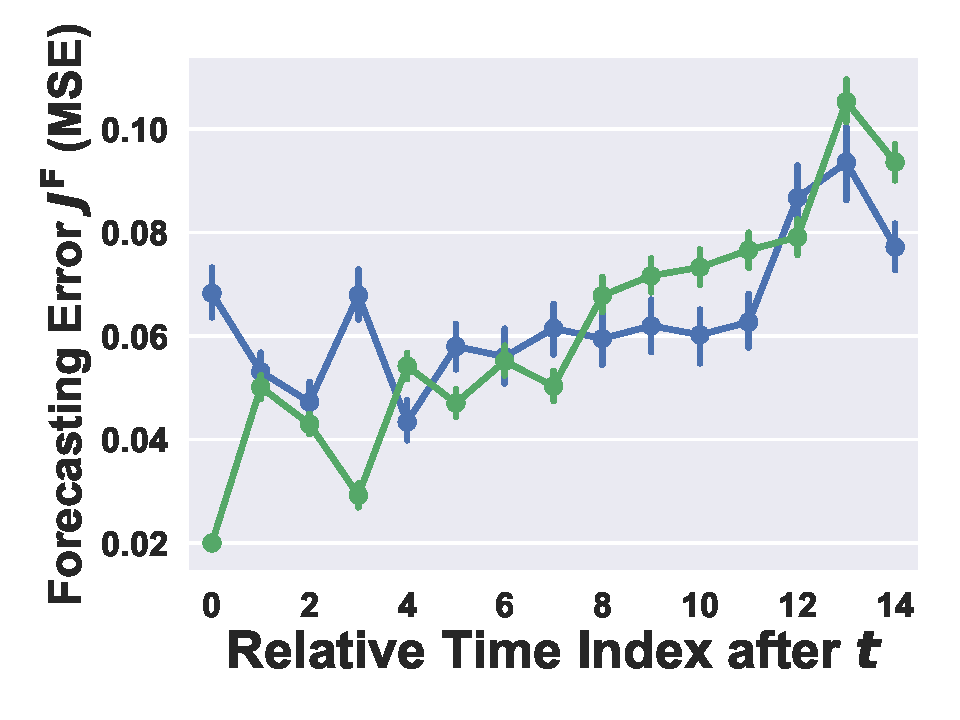
\includegraphics[width=0.31\columnwidth]{figures/iot/forecast_errors_time_horizon.pdf}}
\label{fig_iot_forecast_errors_time_horizon}
}
%\subfigure[]{
\subfigure{
{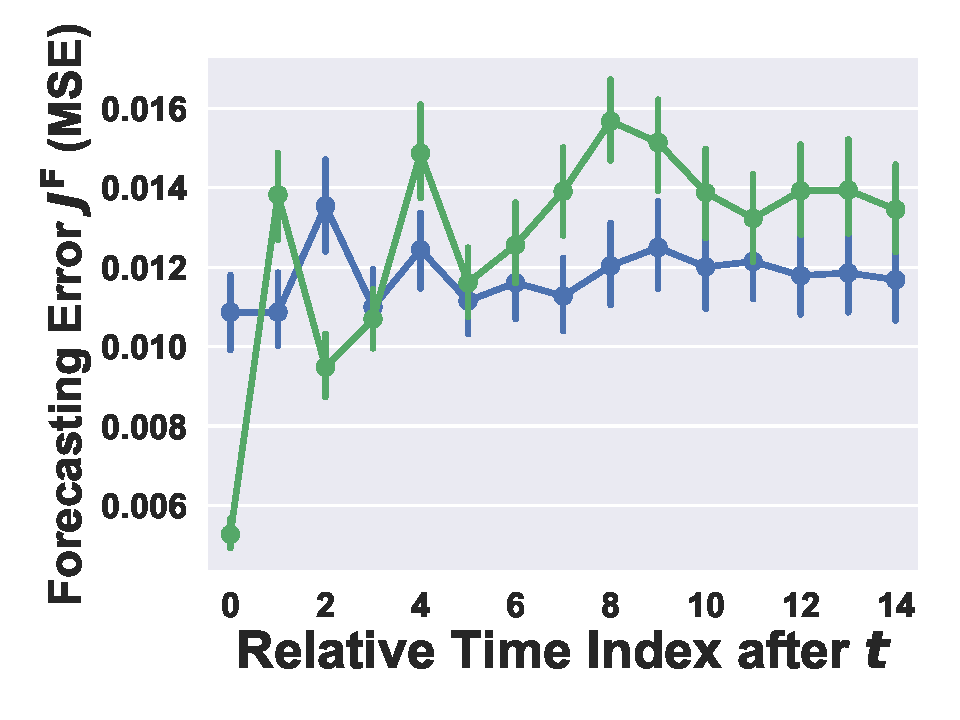
\includegraphics[width=0.31\columnwidth]{figures/cell/forecast_errors_time_horizon.pdf}}
\label{fig_cell_forecast_errors_time_horizon}
}
%\subfigure[]{
\subfigure{
{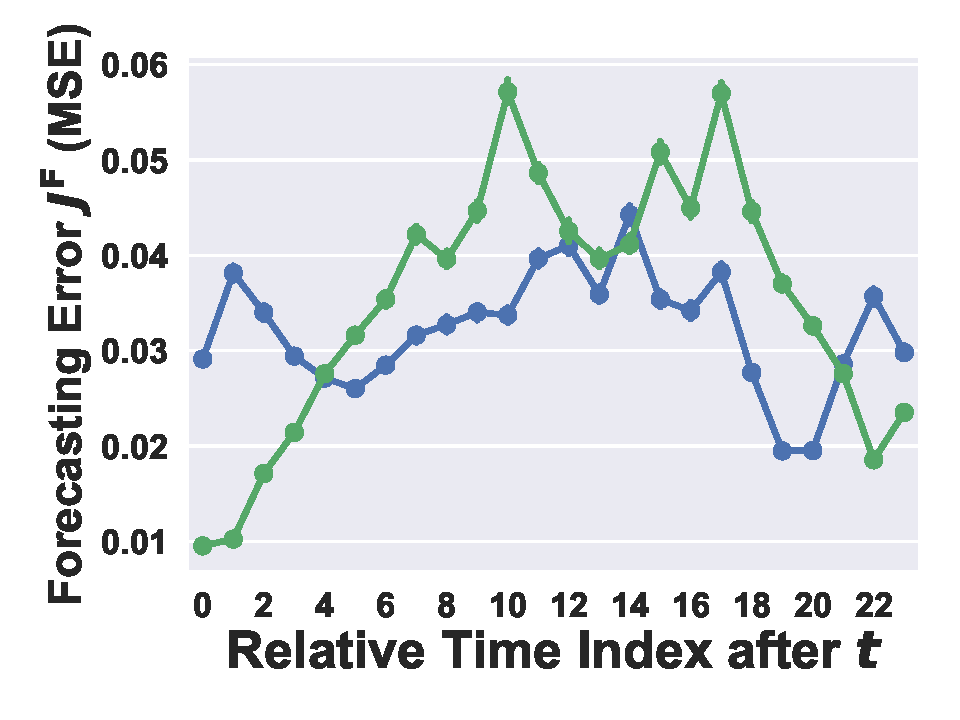
\includegraphics[width=0.31\columnwidth]{figures/pjm/forecast_errors_time_horizon.pdf}}
\label{fig_pjm_forecast_errors_time_horizon}
}
\caption{\textbf{Real-world dataset results: } From left to right, the columns correspond to smart factory regulation from IoT sensors, taxi dispatching with cell demand, and battery storage optimization. \textbf{(Row 1)} Co-design achieves lower cost $\Jcontrol$ for smaller bottlenecks $\zbottleneck$ compared to task-agnostic methods. \textbf{(Row 2)} We also achieve lower error for each dimension $i$ of the vector control, $u(i)$, plotted for a highly-compressed $Z=3$. \textbf{(Row 3)} Co-design heavily reduces forecasting errors for initial horizons that are especially important for MPC's decision-making.}
%While a task-agnostic approach (blue) distributes forecasting errors roughly evenly across a horizon $H$, our co-design approaches heavily reduce errors for initial horizons that are especially important for MPC's decision-making.}
\label{fig_real}
\end{center}
\vskip -0.2in
\end{figure*}
%Aggregated forecasting error for  each relative time index when $Z=3$, under different policies. (j-l) Forecasting error for each $s(i)$ and each relative time index when $Z=3$, under task-agnostic (top) and weighted (bottom) policy, respectively.
%\caption{Results for real data. Columns from left to right corresponds to smart home regulation, taxi dispatching and battery storage optimization, respectively. (a-c) Control cost $J$ under different bottleneck dimension $Z$ and training policies; (d-f) Control error for each $u(i)$ when $Z=3$ under different training policies; (g-i) Aggregated forecasting error for  each relative time index when $Z=3$, under different policies. (j-l) Forecasting error for each $s(i)$ and each relative time index when $Z=3$, under task-agnostic (top) and weighted (bottom) policy, respectively.}


We now evaluate our algorithms on the IoT, taxi scheduling, and battery charging scenarios described in Sec. \ref{sec:scenarios}. Our results on a \textit{test} dataset are depicted in Fig. \ref{fig_real}, where each column corresponds to a real dataset and each row corresponds to an evaluation metric, as discussed below.

\textbf{How does compression affect control cost?} The first row of Fig. \ref{fig_real} quantifies the control cost $\Jcontrol$ for various compressed representations $\zbottleneck$. The optimal cost, in a dashed black line, is an unrealizable lower-bound cost when the controller is given the true future $s_{t:t+H-1}$ without any forecast error. The vertical bars show the distribution of costs across several test rollouts, each with different timeseries $\bolds$. 
%\JC{The vertical bars indicate the distribution of costs across different testing samples.}
%Our key result is that our co-design schemes (green and orange) achieve within \SC{$5 \%$} of the optimal cost but with a representation size that is at least \SC{$4\times$} smaller than a task-agnostic baseline in blue. Thus, for only \SC{$5 \%$} more cost than the optimal scheme, we achieve a compression gain of \SC{$15 \times, 15 \times$}, and \SC{$96 \times$} for the IoT, traffic, and battery datasets respectively. 
% In all curves, our weighted co-design approach (green) requires a marginally larger bottleneck than the purely task-aware approach ($\lambdaforecast = 0$) since the latent representation should minimize both control and forecast error. 
%The benefits of a weighted approach to also minimize forecast error are described subsequently.
Our key result is that our task-aware scheme (orange) achieves within $5 \%$ of the optimal cost, but with a small bottleneck size $Z$ of $4$, $4$ and $2$ for the IoT, traffic, and battery datasets, respectively. This corresponds to an absolute compression gain of $15\times$, $15\times$, and $96\times$ for each dataset. In contrast, with the same bottleneck sizes, a competing task-agnostic scheme (blue) incurs at least $25\%$ more control cost than our method.

Moreover, for the IoT and battery datasets, the task-agnostic benchmark requires a large bottleneck of $Z=35$ and $Z=11$, leading our approach to transmit $88 \%$ and $82 \%$ less data respectively. Strikingly, even for a large representation of $Z = 60$, a task-agnostic scheme incurs $100\%$ more cost than the optimal for the cell traffic dataset. This is because the cost function is highly sensitive to shortages with $\gamma_s \gg \gamma_e$, which is not captured by simply optimizing for \textit{mean} error. To clearly see the trend in Fig. \ref{fig_real}, we only plot until $Z=9$, but ran the experiments until $Z=60$. Our weighted approach (green) requires a marginally larger representation than the purely task-aware approach ($\lambdaforecast = 0$) since it should minimize both control and forecast error. 

\textbf{Does co-design reduce control errors?}
We now investigate how the compression benefits of co-design arise. Given the stochastic nature of all our real world datasets, all prediction models inevitably produce forecasting error, which in turn induce errors in selecting controls. However, the key benefit of co-design methods is they explicitly model and account for how MPC chooses controls based on noisy forecasts $\boldshat$, and are thus able to minimize the control error, which we now quantify.

As defined in Sec. \ref{subsec:input_driven_LQR}, for any state $x_t$, $u_t$ is the optimal first MPC control given perfect knowledge of $s_{t:t+H-1}$, while $\hat{u}_t$ is MPC's actual enacted control given a noisy forecast.
%First, we define the optimal control $u_t$ to be the control selected by MPC given the ground-truth future $s_{t:t+H-1}$ from a given initial state $x_t$. For the same initial condition $x_t$, we define $\hat{u}_t$ to be MPC's control when it is given a forecast $\shat_{t:t+H-1}$ which can have errors due to encoding/decoding. 
Then, the \textit{control errors} across various control dimensions $i$ are the MSE error $\doublevert u_t(i)  - \hat{u}_t(i) \doublevert^2_2$ between optimal control $u_t(i)$ and $\hat{u}_t(i)$. The second row of Fig. \ref{fig_real} clearly shows that our task-aware and weighted methods (orange and green) achieve lower \textit{control} error on all three datasets.

\textbf{Why does co-design yield task-relevant forecasts?} 
To further show that our co-design approach reduces forecasting error for the purposes of an ultimate control task, we show forecasting errors across various time horizons in the third row of Fig. \ref{fig_real}. As argued in the previous section, all forecasting models produce prediction error. However, a task-agnostic forecast (blue) roughly equally distributes prediction error across the time horizon $t$ to $t+H-1$. In stark contrast, the weighted co-design approach (green) drastically reduces prediction errors in the \textit{near future} since MPC enacts the first control $u_t$ and then re-plans on a rolling horizon. Of course, the full forecast $\shat_{t:t+H-1}$ matters to enact control plan $\hat{u}_{t:t+H-1}$, but the cost is most sensitive to the initial forecast and control errors in our MPC scenarios. For visual clarity, we present forecast errors of the fully task-aware approach ($\lambdaforecast = 0$) in the supplement, since the errors are much larger than the other two methods. 
%\SC{discuss 12 hours period battery.}

\subsection{Nonlinear Dynamics with Transition Noise}
\label{subsec:nonlinear}

% \begin{figure}[ht]
% \vskip 0.2in
% \begin{center}
% \subfigure{
% {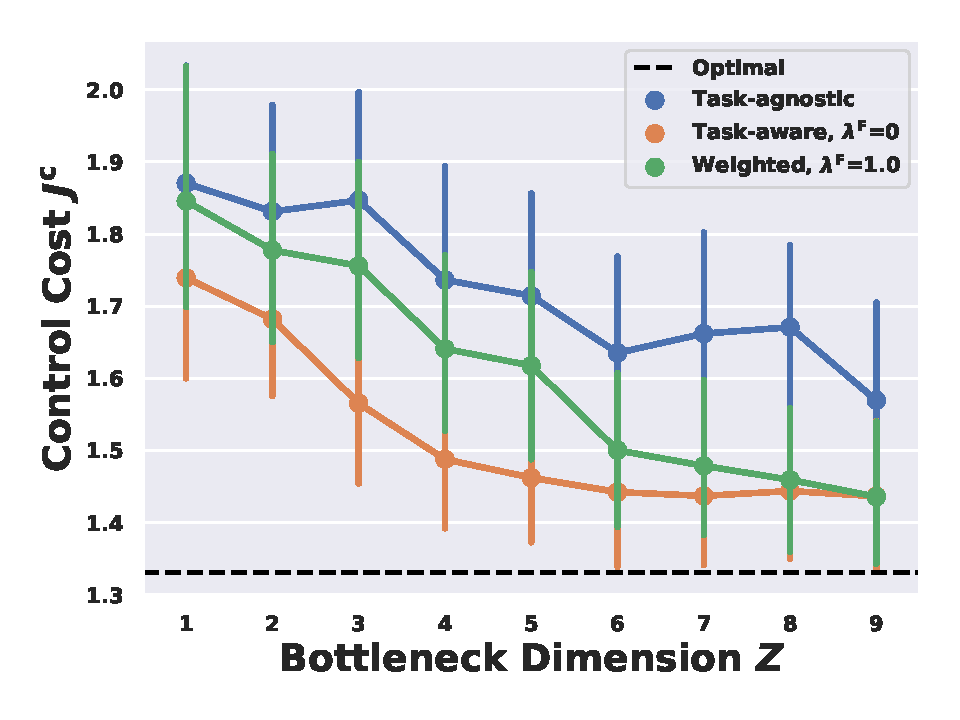
\includegraphics[width=0.6\columnwidth]{figures/video/video_cost_bottleneck.pdf}
% }}
% \caption{Co-Design Results with \textit{Nonlinear} Dynamics and Transition Noise.}
% \label{fig:nonlinear}
% \end{center}
% \vskip -0.2in
% \end{figure}

\begin{wrapfigure}{R}{0.5\columnwidth}
\centering
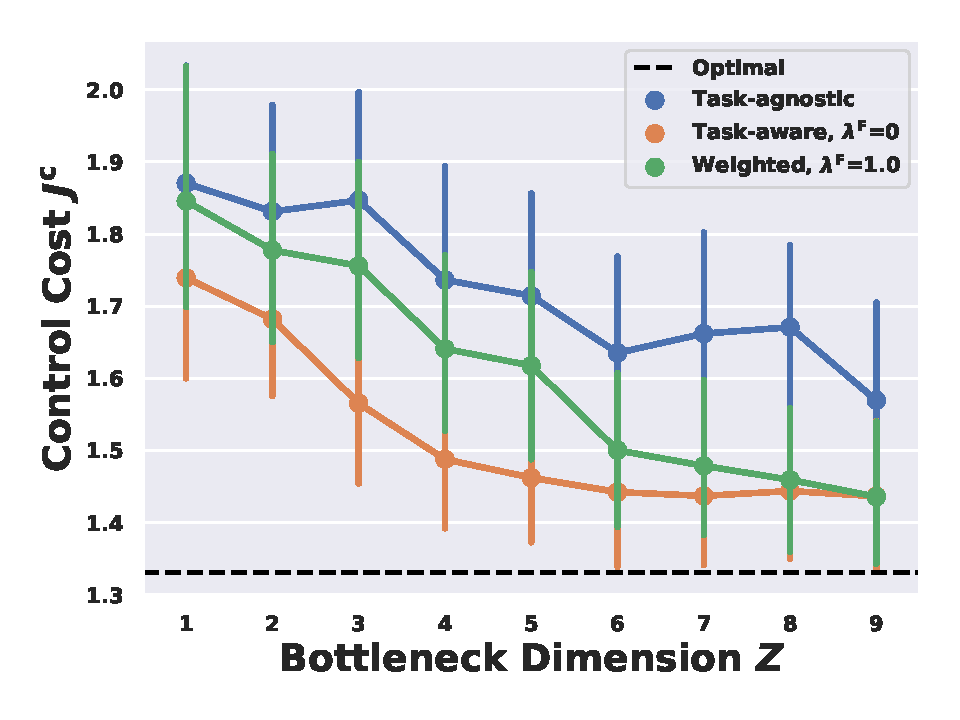
\includegraphics[width=0.5\columnwidth]{figures/video/video_cost_bottleneck.pdf}
\caption{Co-Design Results with \textit{Nonlinear} Dynamics and Transition Noise.}
\label{fig:nonlinear}
% \vskip -0.5em
\end{wrapfigure}


To illustrate that our co-design approach works well for systems with \textbf{nonlinear and stochastic} dynamics, we also provide a nonlinear
example concerning an idealized mobile video streaming scenario. In this application, a mobile video client stores a buffer of video segments and must choose a video quality to download for the next segment of video. The goal is to maximize the quality of video while minimizing video stalls, which occur when the buffer under-flows while waiting for a segment to be downloaded. Here, state $x_t$ represents the buffer of stored video segments, control $u_t$ is segment quality, and $s_t$ is network throughput. The nonlinear dynamics are $x_{t+1} = [ x_{t} - u_t \oslash s_t ]_+ + L_x + \eta_{t}$, where $\oslash$ represents element-wise division, $L_x$ is the increase in stored video for each download, and $\eta_t$ is Gaussian transition noise. The cost aims to keep a positive buffer and have high video quality:
    $\Jcontrol(\boldx, \boldu) = \sum_{t=0}^{T} \gamma_x \doublevert x_t - L_x \doublevert^2_2  + \sum_{t=0}^{T-1} \gamma_u \doublevert u_t - L_u\doublevert^2_2.$

Fig. \ref{fig:nonlinear} clearly shows our approach works quite well for a nonlinear scenario with transition noise, which complements the three linear examples in Sec. \ref{subsec:linear}. In the above experiments, the parameters are: $T=60$, $W = H = 15$, $m=n=p=4$, $\gamma_x = 0.25$, $\gamma_u = 1$, $L_x = 0.5 \times \mathbbm{1}_n$, $L_u = 0.2 \times \mathbbm{1}_m$. 

\textbf{Limitations: } \SC{Our work does not automatically learn the optimal bottleneck size $Z$ that minimizes control cost nor necessarily learn a human-interpretable latent representation.} 
%Further, co-design may yield minimal benefits if every timeseries feature is unique and equally-important for control.}
%However, as evidenced by our evaluation, such a scenario is unlikely for diverse engineering domains.}

